\section{Document Frequency $F_{\mathcal{D},q}$}

In this section we will see how to efficiently compute the document frequency $F_{\mathcal{D},q}$ for a given query $q$ following a method from Sadakane \cite{Sadakane2007}.

\begin{Definition}
  The \defi{binary generalized suffix tree}{Binary Generalized Suffix Tree} (\id{BGST}) of a text is the suffix tree with inserted inner nodes, such that the each vertex has degree $0$ or $2$. Figure~\ref{fig:binaryGeneralizedSuffixTreeExample} shows the \id{BGST} for \texttt{LA O LA \# O LA LA LA \# O O LA \# \$}.
\end{Definition}

To count the document frequency $F_{\mathcal{D},q}$, execute the following steps:
\begin{enumerate}
  \item Build the \id{BGST}.
  \item For each inner node $v$ in \id{BGST} keep a list $L_v$ of repeated documents. A document $d$ is added to $L_v$, if $d$ occurs in a leaf of the left and of the right subtree.
  \item For a pattern $q$ let $v_q$ be the \defi{locus}{Locus}, that is the lowest node which path is prefixed by $q$. $F_{\mathcal{D},q}$ equals the number of leaves in the subtree of $v_q$ minus the number of repeated documents ($\sum_{v \in T_{v_q}} \vert L_v \vert$) in $v_q$'s subtree $T_{v_q}$.
\end{enumerate}
To find the number of repeated documents in the subtree of an inner node, number the nodes in order (as in Figure~\ref{fig:binaryGeneralizedSuffixTreeExample}). Traverse in this order and append $\vert L_v \vert$ in unary coding ($\vert L_v \vert$ $0$s and one $1$) to a bitvector $H$, which was initialized with a single $1$. Then all nodes of each possible subtree are contiguous and the number of repeated documents can be calculated by two select queries. This is shown in Algorithm~\ref{alg:documentFrequency}. The runtime depends only on the time to do the backward search.

\begin{figure}[htb]
  \centering
  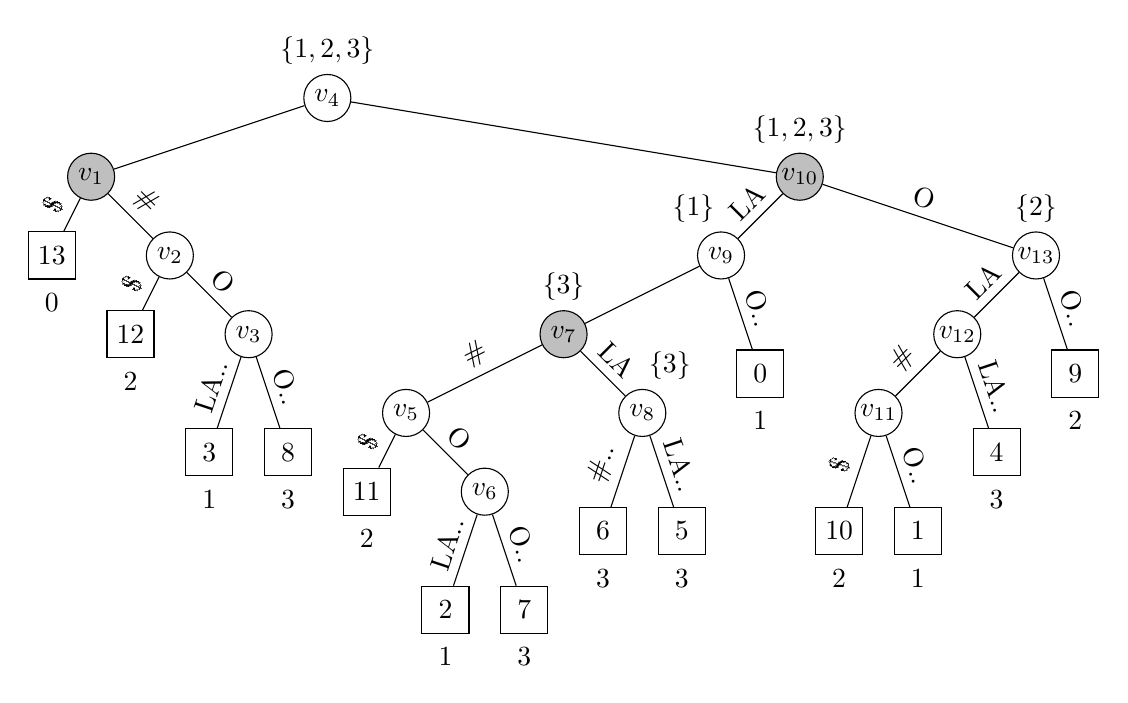
\begin{tikzpicture}[x={(5mm, 0mm)}]
  \tikzstyle{vertex}=[draw,minimum size=17pt, inner sep=0pt]
  \node[vertex, circle] (v4) at (0, 0) {$v_4$};
  \node (l4) at (0, 0.6) {$\{1,2,3\}$};

  \node[vertex, circle, fill=lightgray] (v1) at (-6, -1) {$v_1$};
  \draw (v4) -- (v1);

  \node[vertex, circle] (v2) at (-4, -2) {$v_2$};
  \draw (v1) -- (v2) node[above, sloped, pos=0.5] {\#};

  \node[vertex, circle] (v3) at (-2, -3) {$v_3$};
  \draw (v2) -- (v3) node[above, sloped, pos=0.5] {O};

  \node[vertex, circle, fill=lightgray] (v10) at (12, -1) {$v_{10}$};
  \node (l10) at (12, -0.4) {$\{1,2,3\}$};
  \draw (v4) -- (v10);

  \node[vertex, circle] (v9) at (10, -2) {$v_9$};
  \node (l9) at (9.3, -1.4) {$\{1\}$};
  \draw (v10) -- (v9) node[above, sloped, pos=0.5] {LA};

  \node[vertex, circle, fill=lightgray] (v7) at (6, -3) {$v_7$};
  \node (l7) at (6, -2.4) {$\{3\}$};
  \draw (v9) -- (v7);

  \node[vertex, circle] (v5) at (2, -4) {$v_5$};
  \draw (v7) -- (v5) node[above, sloped, pos=0.5] {\#};

  \node[vertex, circle] (v6) at (4, -5) {$v_6$};
  \draw (v5) -- (v6) node[above, sloped, pos=0.5] {O};

  \node[vertex, circle] (v8) at (8, -4) {$v_8$};
  \node (l8) at (8.7, -3.4) {$\{3\}$};
  \draw (v7) -- (v8) node[above, sloped, pos=0.5] {LA};

  \node[vertex, circle] (v13) at (18, -2) {$v_{13}$};
  \node (l13) at (18, -1.4) {$\{2\}$};
  \draw (v10) -- (v13) node[above, sloped, pos=0.5] {O};

  \node[vertex, circle] (v12) at (16, -3) {$v_{12}$};
  \draw (v13) -- (v12) node[above, sloped, pos=0.5] {LA};

  \node[vertex, circle] (v11) at (14, -4) {$v_{11}$};
  \draw (v12) -- (v11) node[above, sloped, pos=0.5] {\#};

  \node[vertex] (s13) at (-7, -2) {$13$};
  \node (d13) at (-7, -2.6) {$0$};
  \draw (v1) -- (s13) node[above, sloped, pos=0.5] {\$};

  \node[vertex] (s12) at (-5, -3) {$12$};
  \node (d12) at (-5, -3.6) {$2$};
  \draw (v2) -- (s12) node[above, sloped, pos=0.5] {\$};

  \node[vertex] (s3) at (-3, -4.5) {$3$};
  \node (d3) at (-3, -5.1) {$1$};
  \draw (v3) -- (s3) node[above, sloped, pos=0.5] {LA..};

  \node[vertex] (s8) at (-1, -4.5) {$8$};
  \node (d8) at (-1, -5.1) {$3$};
  \draw (v3) -- (s8) node[above, sloped, pos=0.5] {O..};

  \node[vertex] (s11) at (1, -5) {$11$};
  \node (d11) at (1, -5.6) {$2$};
  \draw (v5) -- (s11) node[above, sloped, pos=0.5] {\$};

  \node[vertex] (s2) at (3, -6.5) {$2$};
  \node (d2) at (3, -7.1) {$1$};
  \draw (v6) -- (s2) node[above, sloped, pos=0.5] {LA..};

  \node[vertex] (s7) at (5, -6.5) {$7$};
  \node (d7) at (5, -7.1) {$3$};
  \draw (v6) -- (s7) node[above, sloped, pos=0.5] {O..};

  \node[vertex] (s6) at (7, -5.5) {$6$};
  \node (d6) at (7, -6.1) {$3$};
  \draw (v8) -- (s6) node[above, sloped, pos=0.5] {\#..};

  \node[vertex] (s5) at (9, -5.5) {$5$};
  \node (d5) at (9, -6.1) {$3$};
  \draw (v8) -- (s5) node[above, sloped, pos=0.5] {LA..};

  \node[vertex] (s0) at (11, -3.5) {$0$};
  \node (d0) at (11, -4.1) {$1$};
  \draw (v9) -- (s0) node[above, sloped, pos=0.5] {O..};

  \node[vertex] (s9) at (19, -3.5) {$9$};
  \node (d9) at (19, -4.1) {$2$};
  \draw (v13) -- (s9) node[above, sloped, pos=0.5] {O..};

  \node[vertex] (s4) at (17, -4.5) {$4$};
  \node (d4) at (17, -5.1) {$3$};
  \draw (v12) -- (s4) node[above, sloped, pos=0.5] {LA..};

  \node[vertex] (s10) at (13, -5.5) {$10$};
  \node (d10) at (13, -6.1) {$2$};
  \draw (v11) -- (s10) node[above, sloped, pos=0.5] {\$};

  \node[vertex] (s1) at (15, -5.5) {$1$};
  \node (d1) at (15, -6.1) {$1$};
  \draw (v11) -- (s1) node[above, sloped, pos=0.5] {O..};
\end{tikzpicture}

  \caption{The binary generalized suffix tree of an example document collection $\mathcal{D} = \texttt{LA O LA \# O LA LA LA \# O O LA \# \$}$. The filled vertices are the dummy nodes added to get a binary tree. Round nodes are inner nodes, square nodes are leaves corresponding to suffixes. The number below each leaf is the entry in the document array.}
  \label{fig:binaryGeneralizedSuffixTreeExample}
\end{figure}

\begin{algorithm}[htb]
  \begin{codebox}
    \Procname{$\proc{Document-Frequency}(q)$}
    \li $[l,r] \gets \proc{Backward-Search(\id{CSA}, q)}$
    \li $s \gets r - l + 1$
    \li $y \gets \proc{Select}_1(r, H)$
    \li \If $l \isequal 0$
        \Then
    \li   \Return $s - (y - r + 1)$
    \li \Else
    \li   $x \gets \proc{Select}_1(l, H)$
    \li   \Return $s - (y - r + 1 - (x - l + 1))$
        \End
  \end{codebox}
  \caption{Compute the document frequency $F_{\mathcal{D},q}$ for query $q$.}
  \label{alg:documentFrequency}
\end{algorithm}

\begin{Example}
  Figure~\ref{fig:binaryGeneralizedSuffixTreeExample} shows the \id{BGST} for \texttt{LA O LA \# O LA LA LA \# O O LA \# \$}. We get the following bitvector $H$:
  \begin{align*}
    H = 1
    \underbrace{1}_{v_1}
    \underbrace{1}_{v_2}
    \underbrace{1}_{v_3}
    \underbrace{0001}_{v_4}
    \underbrace{1}_{v_5}
    \underbrace{1}_{v_6}
    \underbrace{01}_{v_7}
    \underbrace{01}_{v_8}
    \underbrace{01}_{v_9}
    \underbrace{0001}_{v_{10}}
    \underbrace{1}_{v_{11}}
    \underbrace{1}_{v_{12}}
    \underbrace{01}_{v_{13}}
  \end{align*}
  Let's now consider $q = \texttt{LA}$. Then \proc{Backward-Search} returns suffix array interval $[4,9]$. Executing the steps in Algorithm~\ref{alg:documentFrequency} yields $s = 6$, $y = 15$ and $x = 7$, so that $3$ is returned.
\end{Example}

\begin{Theorem}
  The document frequency can be calculated with an index needing $\mathcal{O}(n + \vert \id{CSA} \vert)$ bits space.
\end{Theorem}

\begin{Proof}
  The bitvector $H$ has maximum size $2n - N$. Additionally $o(n)$ bits for a constant time select structure are needed. The only thing left is the space needed for \id{CSA}.
\end{Proof}
